\subsection{AeroValve}
\subsubsection{AeroValve Design - Coby Jacobs}
\label{AeroValveDesign}
The AeroValve is a unique feature to this SFRJ. This component came from the goal to decrease the velocity of the axial flow in the combustion chamber. The axial flow needs to be controlled in the combustion chamber to enhance flameholding capabilities. Specifically, if the Mach number in the chamber reached 0.76 the flame would extinguish. With the AeroValve, the flow from the inlet is separated, allowing for some axial flow in the combustion chamber and bringing some of the air through the AeroValve so that it can be distributed radially to slow down the flow and improve flameholding. The system is designed such that 40\% of the air is allowed to flow from the inlet into the combustion chamber and 60\% of the air flows into the AeroValve.The AeroValve has four injection port locations plus and end port. The injection ports are evenly distributed along the AeroValve. Fig. (\ref{fig:isometric}) shows an isometric view of the AeroValve, Fig. (\ref{fig:intake}) shows a view of the AeroValve intake, and Fig. (\ref{fig:bypassflow})

\begin{figure}[H]
    \centering
    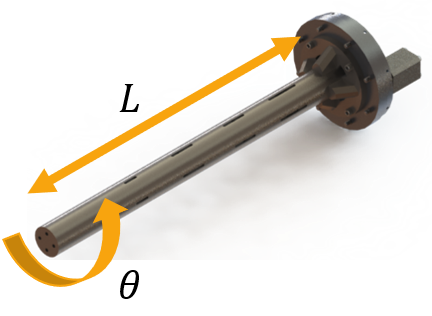
\includegraphics[width=0.7\linewidth]{Combustor_Figures/isometric.png}
    \caption{AeroValve isometric view}
    \label{fig:isometric}
\end{figure}

\begin{figure}[H]
    \centering
    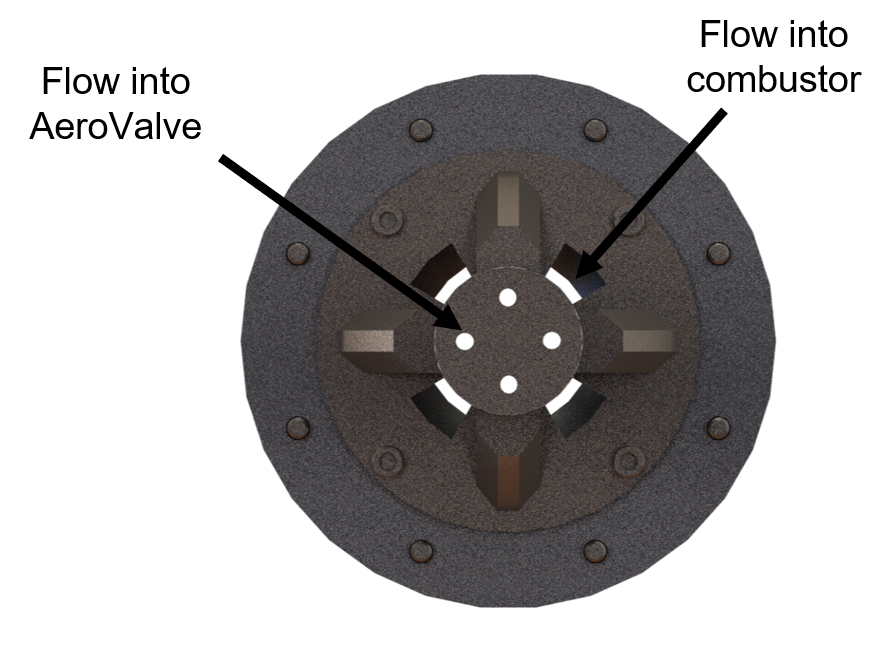
\includegraphics[width=0.7\linewidth]{AeroValve_Figures/bypass_intake.png}
    \caption{AeroValve intake}
    \label{fig:intake}
\end{figure}

\begin{figure}[H]
    \centering
    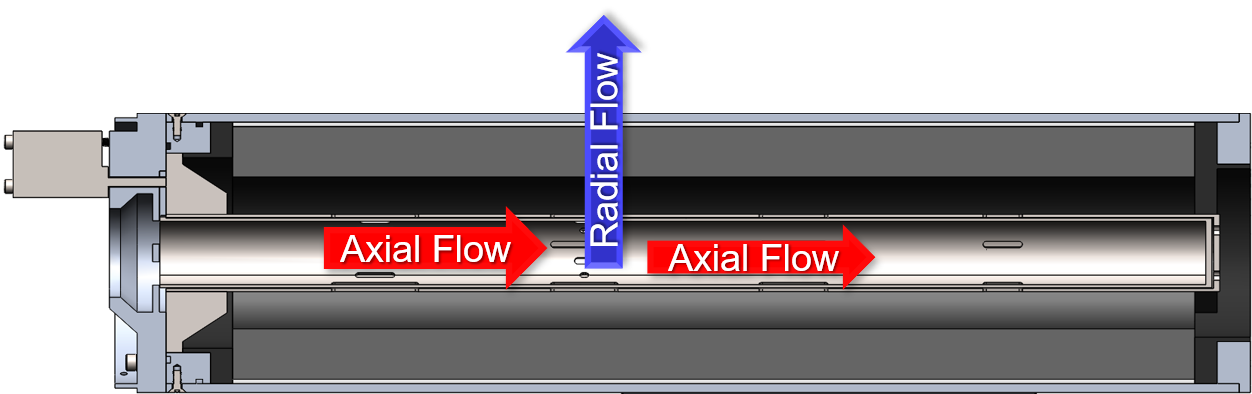
\includegraphics[width=0.7\linewidth]{AeroValve_Figures/bypass_flow.png}
    \caption{AeroValve flow}
    \label{fig:bypassflow}
\end{figure}

The AeroValve provides throttling by consisting of two concentric tubes, each with slots that can be aligned by the inner tube rotating a prescribed set of degrees to provide the needed mass flow. There are three scheduled settings for the position of the inner tune at ignition, cruise, and maneuver. 

The AeroValve was sized for the flow in the inner tube to be Mach 0.8. The inner diameter of the central valve for this condition is 1.43".  

\begin{figure}[H]
    \centering
    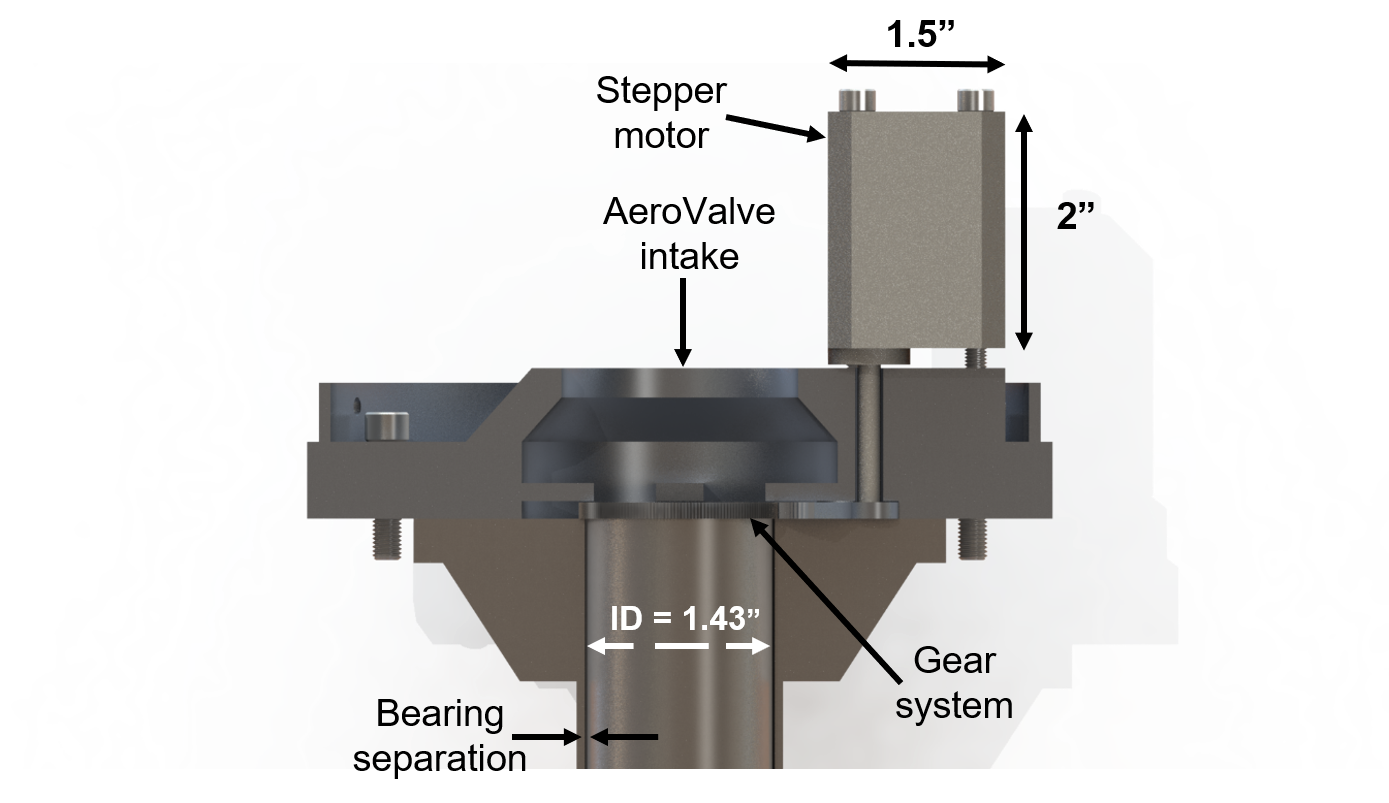
\includegraphics[width=0.7\linewidth]{Combustor_Figures/topview.png}
    \caption{AeroValve top view}
    \label{fig:topview}
\end{figure}

\subsubsection{AeroValve Actuation - Coby Jacobs}

In order to rotate the central tube of the AeroValve system, a gear actuation system had to be designed. The requirements of the actuation system were derived from eq. (\ref{torque_1}). It is assumed that there is negligible friction force between the two valves due to the use of bearings.

\begin{equation}
\centering   
\tau=I\alpha
\label{torque_1}
\end{equation}

This equation was be integrated twice with respect to time to so that a prescribed angle to rotate and time could be used to calculate torque.

\begin{equation}
\centering   
\tau=\frac{2I\alpha}{t^2}
\end{equation}

The moment of inertia of the valve was found using eq. (\ref{moment_inertia}).

\begin{equation}
    \centering
    I = \frac{\pi\rho h}{2}(r_2^4-r_1^4)
    \label{moment_inertia}
\end{equation}

Initially assuming that the tube would be made of steel and would have the maximum allowable dimensions in the chamber, the moment of inertia was estimated to be 0.01205 $kg-m^4$. Using this, a basic assumption to turn $60\deg$ in one second, and a large factor of safety, the required torque is 0.1 N-m, or .074 ft-lbs.

With a relatively small torque requirement, a small stepper motor can be used to control the gears. A large gear can be fitted around the AeroValve, but because the motor is much smaller than the large gear, the largest gear that can fit on the motor to be the driving gear will not be large enough to come in contact with the large driven gear. Due to this, future work will need to be done in the detailed mechanical design of the gear train so that a third gear can be fitted into the system.

\subsubsection{AeroValve Flow Analysis-Ariana Martinez}
The AeroValve flow analysis was divided between axial flow going through the AeroValve tube, and radial injected flow going into the combustor. both flows were analyzed under the assumptions of 1-D steady state incompressible flow with constant temperature. It is acknowledged that the initial mach in the AeroValve tube is 0.8 and incompressible flow is a poor assumption to make. However, the purpose of doing and analysis on the AeroValve was to assess its impact on the overall flight performance and thus it was desired to have a set of equations that could be solved analytically within the simulator. Due to having split mass flows, characterization of the AeroValve flow with compressibility effects will need to be conducted using a 2-D CFD model.This is an area of future work. A control volume of the axial flow is shown below in fig. \ref{fig:AeroValveAxialCV}.

\begin{figure}[H]
 \centering
    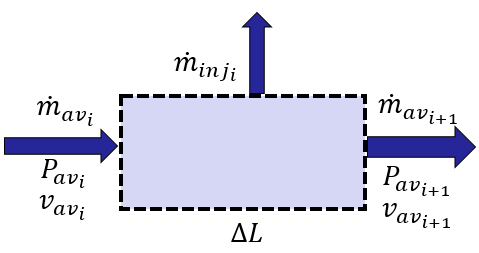
\includegraphics[width=0.5\linewidth]{AeroValve_Figures/AeroValveAxialCV.PNG}
    \caption{AeroValve Control Volume}
    \label{fig:AeroValveAxialCV}
\end{figure}

In this control volume, \textit{i} is a differential step down the combustor. The bypass analysis was discretized down the combustor and performed in tandum with the descrized combustor analysis.At the inlet of the AeroValve tube, \(i=1\),mass flow into the AeroValve,\(\dot{m}_{av}\) is set by
\begin{equation}
    \centering
    \dot{m}_{av}=Percent Bypass*\dot{m}_{inlet}
\end{equation}

The optimal percent of air bypassing the combustor to flow into the AeroValve was determined from paramater sweeps to be 60\% bypass. The pressure,\(P_{av}\), temperature, \(T_{av}\), velocity, \(v_{av}\),and density,\(\rho_{av}\) were set equal to corresponding inlet conditions.  

The injection mass flow rate, \(\dot{m}_{inj}\) going out of each injection port was set as the desired percentage of AeroValve flow to be distributed to each port. If there is no port at a location, \textit{i}, then injection mass flow percentage is set to zero. Eq.(\ref{mdot injection}) shows how each injection mass flow is calculated, where each element in the array represents the location corresponding to \textit{i} along the combustor.  
\begin{equation}
    \centering
\dot{m}_{inj}= \dot{m}_{av}*
[0 \hspace{2mm} 0 \hspace{2.5mm} \% \hspace{0.5mm} port \hspace{0.5mm} 1 \hspace{2.5mm}
 0 \hspace{2mm} 0 \hspace{2.5mm} \% \hspace{0.5mm} port \hspace{0.5mm} 2 \hspace{2.5mm}
 0 \hspace{2mm} 0 \hspace{2.5mm} \% \hspace{0.5mm} port \hspace{0.5mm} 3 \hspace{2.5mm}
 0 \hspace{2mm} 0 \hspace{2.5mm} \% \hspace{0.5mm} port \hspace{0.5mm} 4 \hspace{2.5mm} 
 0 \hspace{2mm} 0 \hspace{2.5mm} \% \hspace{0.5mm} end  \hspace{0.5mm} port]
 \label{mdot injection}
\end{equation}
The design criteria for determining a desired flow distribution through each port will be discussed the the Actuation Schedule section.
Thus, mass flow in the aerovalve tube at each location was calculated by mass conservation in eq.(\ref{bypass mdot})
\begin{equation}
    \centering
    \dot{m}_{av_{i+1}}= \dot{m}_{av_{i}}- \dot{m}_{inj_{i}}
     \label{bypass mdot}
\end{equation}
and velocity in the AeroValve at each port location, \(v_{av_{i+1}}\) is given by Continuity in eq.(\ref{bypass velocity}), where \(A_{av}\) is the cross sectional area of the inside of the bypass tube, and \(\rho_{air}\) is the air density at the end of the inlet.  
\begin{equation}
    \centering
    v_{av_{i+1}}= \frac{\dot{m}_{av_{i+1}}}{A_{av}\rho_{air}}
    \label{bypass velocity}
\end{equation}
it was assumed that there was no work or heat transferred in or out of the system. Thus, if \(\dot{m}_{inj}\) at a location \textit{i} was zero, then the static pressure in the Aerovalve tube, \(P_{av}\) at each location is given by eq.(\ref{bypass pressure 1})

\begin{equation}
    \centering
    P_{av_{i+1}}=P_{av_{i}}
\end{equation}
if \(\dot{m}_{inj}\) is nonzero at \textit{i}, then momentum balance on the control volume states:
\begin{equation}
    \centering
    P_{av_{i+1}}=P_{comb_{i}}
    \label{bypass pressure 1}
\end{equation}
where \(P_{comb}\) is the combustor static pressure at the location, \textit{i}.

Characterizing the flow properties down the Aerovalve tube allows us to characterize the flow of injected air into the combustor. The control volume for injected air is shown below in fig.\ref{fig:AeroValveInjectionCV}.

\begin{figure}[H]
 \centering
    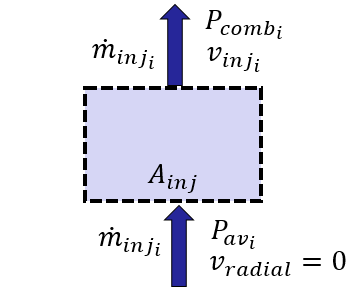
\includegraphics[width=0.5\linewidth]{AeroValve_Figures/AeroValveInjectionCV.PNG}
    \caption{Injection Port Control Volume}
    \label{fig:AeroValveInjectionCV}
\end{figure}
it is assumed that in the AeroValve, radial velocity, \(v_{radial}\)is zero. because of the incompressible flow assumption, the radial velocity of injected mass flow from the AeroValve into the combustor,\(v_{inj}\) can be computed at a location,\textit{i} using eq.(\ref{discharge vel})

\begin{equation}
    \centering
    v_{inj_{i}}=\sqrt{2\rho_{air}(P_{av_i}-P_{comb_i})}
    \label{discharge vel}
\end{equation}
The injection port area,\(A_{inj}\), can then calculated at each location to accommodate the desired mass flow using Continuity in eq.(\ref{discharge area})
\begin{equation}
    A_{inj_i}=\frac{\dot{m}_{inj}}{\rho_{air}v_{inj_i}}
    \label{discharge area}
\end{equation}
These equations for solving the axial and radial flow of air in the AeroValve are looped in the simulator both down the combustor and with time. At each iteration down the combustor, the injected air mass flow is passed to the combustor code and the flow properties in the combustor are updated.

\subsubsection{Actuation Schedule-Ariana Martinez}
In order to meet all design requirements, it was desired to have airflow that was optimized for each state of flight. the flight states that were identified were ignition state, cruise state, and maneuver state\newline
\newline
    \underline{ Ignition State}\newline
    the goal during ignition was to be able to sustain the flame. this was achieved by injecting a large amount of radial flow in the front of the combustor in order to create re-circulation  of the flow. Flameholding will be discussed in detail in section V.C. Based on this criteria, the distribution of flow through the Aerovalve was selected to be 80\% of air through port 1, 20\% of air through port 2, and all other ports closed.fig.(\ref{fig:unrolled ignition}) shows the hole pattern for ignition phase
\begin{figure}[H]
\centering
  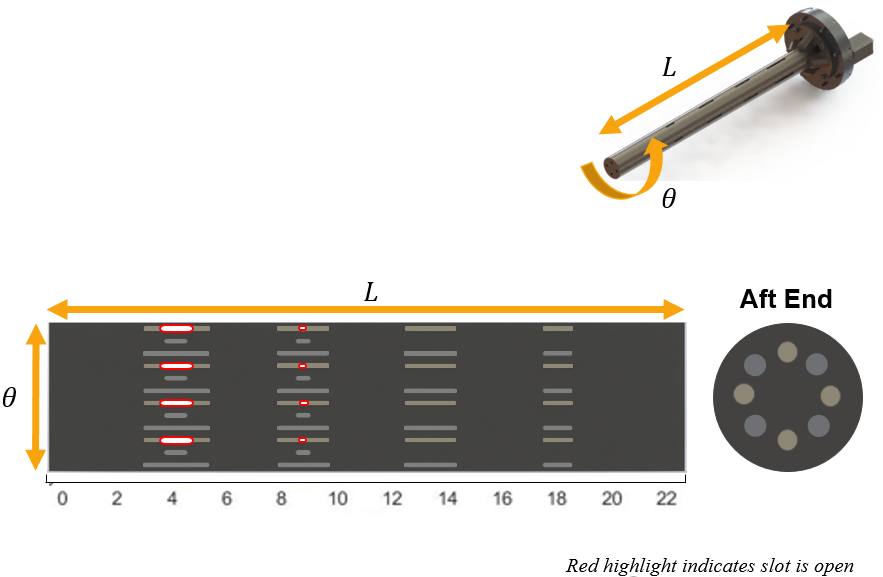
\includegraphics[width=.8\linewidth]{AeroValve_Figures/unrolled_aerovalve_ignition.PNG}
  \caption{Unrolled image of AeroValve Port Alignment during ignition}
  \label{fig:unrolled ignition}
\end{figure}
the corresponding mass flow rates and port sizes are shown below in fig.(xx) and fig. (xx) respectively. 
\begin{figure}[H]
\centering
\begin{minipage}{.5\textwidth}
  \centering
    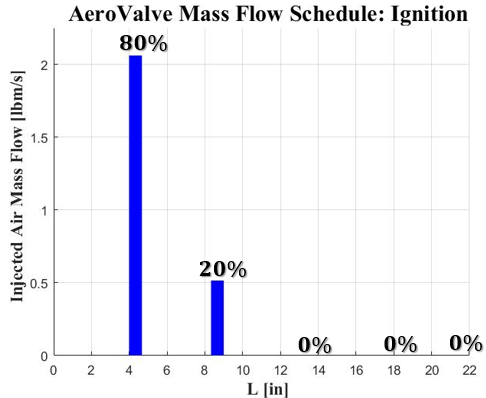
\includegraphics[width=.8\linewidth]{AeroValve_Figures/ignition_port_areas.PNG}
  \captionof{figure}{AeroValve Mass Flow Schedule During Ignition}
  \label{fig:ignition mass flow}
\end{minipage}%
\begin{minipage}{.5\textwidth}
  \centering
  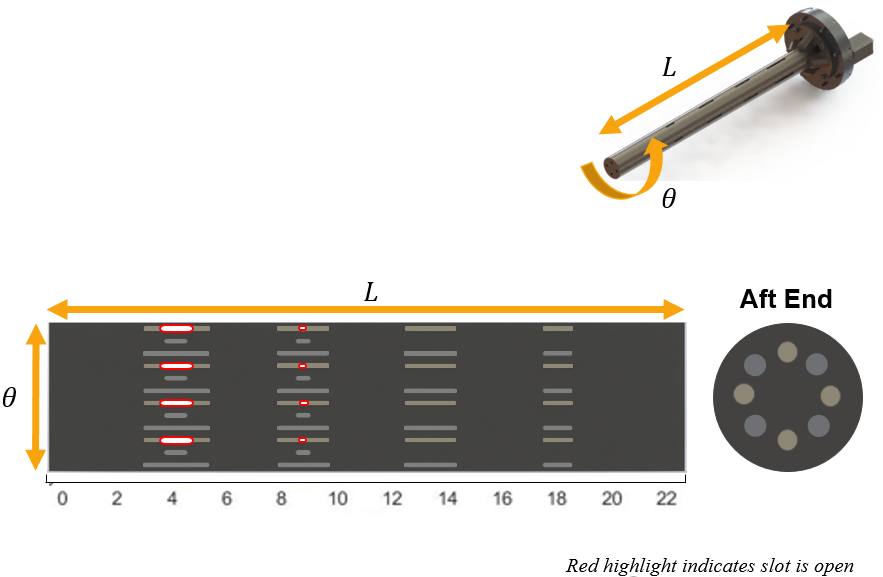
\includegraphics[width=.8\linewidth]{AeroValve_Figures/unrolled_aerovalve_ignition.PNG}
  \captionof{figure} Port Areas During Ignition Phase}
  \label{fig:ignition port area}
\end{minipage}
\end{figure}




the flow properties for the aerovalve and combustor in the ignition phase are shown below in figs. (xx) and (xx)



-ignitor goal and method
-image of rolled out aerovalve
-mass flow and velocity plots
-table of injection areas

-cruise goal and method
-image of rolled out aerovalve
-mass flow and velocity plots
-table of injection areas

-maneuver goal and method
-image of rolled out aerovalve
-mass flow and velocity plots
-table of injection areas

\subsubsection{AeroValue Thermal Analysis-Jonathan Rohwer}

Combustors are extreme environments and building an AeroValve to withstand the temperatures requires an understanding of the heat transfer into and out of the AeroValue. Using the thermal and transport properties from the AeroValue and combustor analysis a steady state solution was found. This solution has a couple of assumptions to simplify the initial analysis: \\
\begin{enumerate}
    \item Neglect axial heat conduction
    \item Neglect radiation
    \item Steady state
    \item Axisymmetric heat transfer
    \item Constant combustor port area \\
\end{enumerate}
The system was modeled as a solid pipe with convective flow on the inside (AeroValve flow) and outside (combustor). For the AeroValve flow, the McAdams pipe flow correlation was used to determine the convective heat transfer coefficient. This equation can be seen in eq.(\ref{McAdams})
\begin{equation}
    h_g=\frac{k_\infty}{D}0.026Re^{0.8}Pr^{0.4}
    \label{McAdams}
\end{equation}
where
\begin{equation}
    Re=\frac{\rho_\infty\nu_\infty D}{\mu_\infty}
\end{equation}
\begin{equation}
    Pr=\frac{\mu_\infty C_{p\infty}}{k_\infty}
\end{equation}
For the combustor flow, a form of the Bartz correlation was used to determine the convective heat transfer coefficient. This equation can be seen in eq.(\ref{Bartz})
\begin{equation}
    h_g=\frac{0.026}{D_h^{0.2}}\Big(\frac{\mu^{0.2}C_p}{Pr^{0.6}}\Big)_0(\rho_\infty U_\infty)^{0.8}\frac{1}{\sigma}
    \label{Bartz}
\end{equation}
where
\begin{equation}
    \sigma=\Big[\frac{1}{2}\frac{T_w}{T_0}\Big(1+\frac{\gamma-1}{2}M^2\Big)+\frac{1}{2}\Big]^{0.68}\Big[1+\frac{\gamma-1}{2}M^2\Big]^{0.12}
\end{equation}
\begin{equation}
    Pr=\frac{\mu_0 C_{p0}}{k_0}
\end{equation}
For Bartz specific units are used:
\begin{itemize}
    \item $C_p=[Btu/lb-\cr F]$
    \item $D_h=[in]$
    \item $T_w=T_0=[\cr R]$
    \item $\rho_\infty=[lb/in^3]$
    \item $U_\infty=[in/s]$
    \item $\mu=[lb/in-s]$
\end{itemize}


\subsubsection{Future Work - Stephen Kubicki}

An alternate design was created for the AeroValve as a potential lighter weight solution, but was not able to be integrated into the GLD simulation as of this paper's writing. A CAD rendition of this design can be seen in Fig. \ref{fig:AeroValve2_Labeled}. The design features rotating and stationary plates at the middle and end of the AeroValve, which control how much flow is apportioned in the fro

Approximate streamlines can also be seen in the figure, drawn in blue and going through the tube perforations.

\begin{figure}[H]
\centering
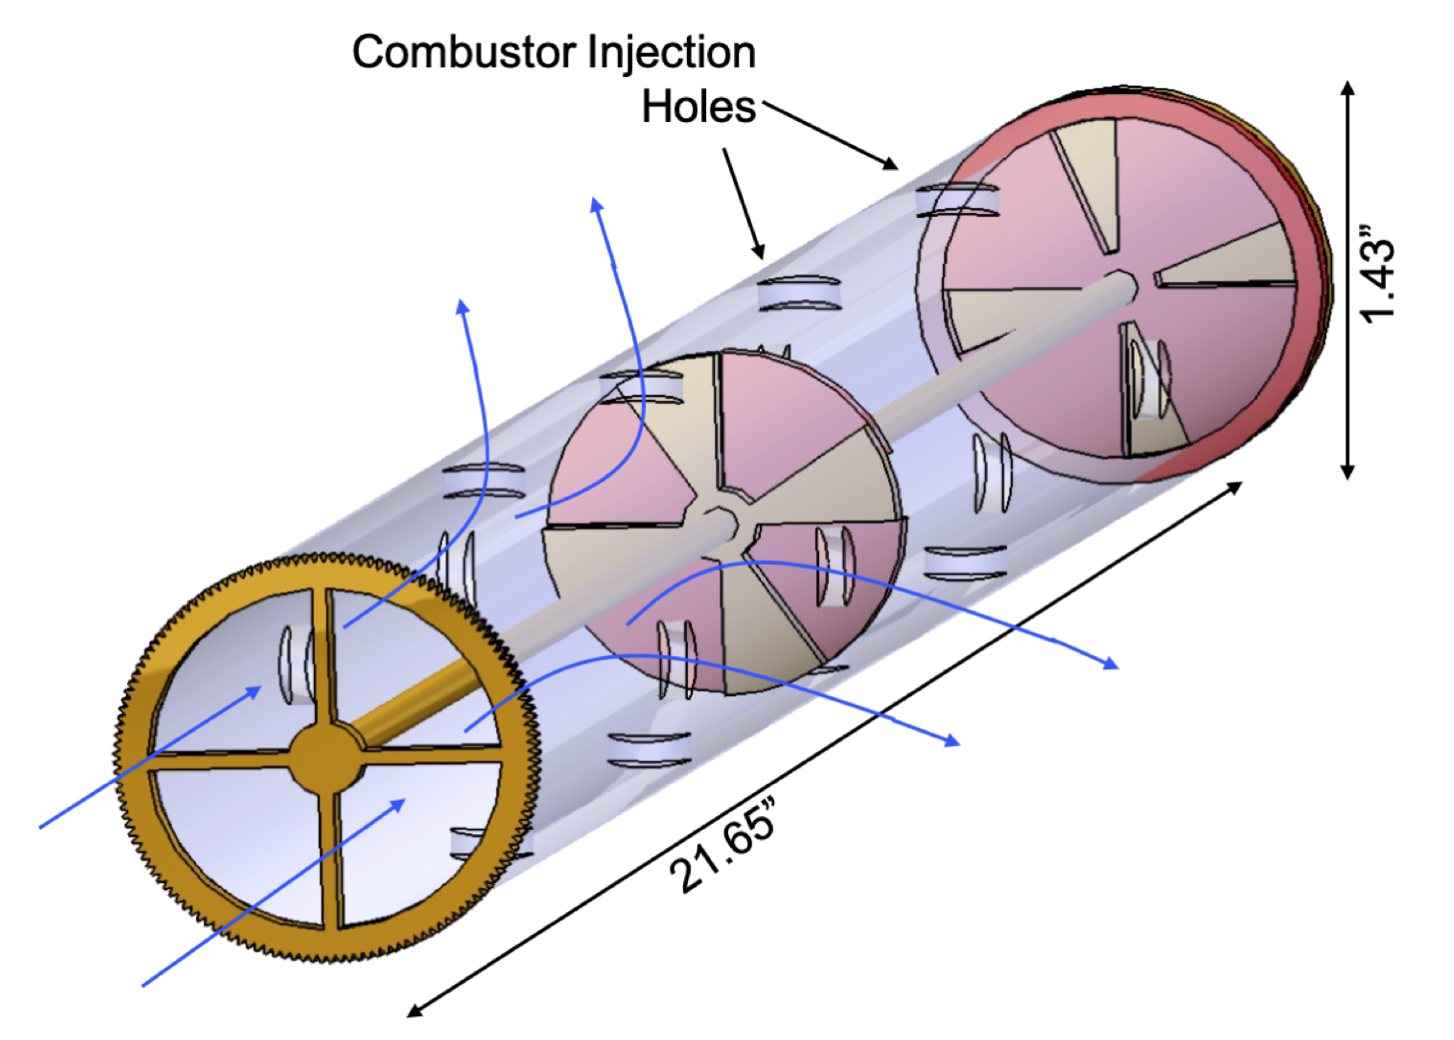
\includegraphics[width=1\textwidth] {AeroValve_Figures/AeroValve2_Labeled.png}
\caption{AeroValve Design Alternative}
\label{fig:AeroValve2_Labeled}
\end{figure}